\chapter{Conclusions}
\label{chConclusions}

The nature of dark matter still remains an unanswered question of modern physics. XENON100 is so far the leading experiment in the field of direct dark matter detection and has achieved the best limits on the spin-independent WIMP-nucleon scattering cross-section above $\sim$10~GeV~\cite{xe100-run08}.
Within this thesis, I have been involved in almost all aspects of the development and operation of the XENON100 detector, characterization with radioactive and external light sources, Monte Carlo simulations and data analysis.

\begin{figure}[!b]
\centering
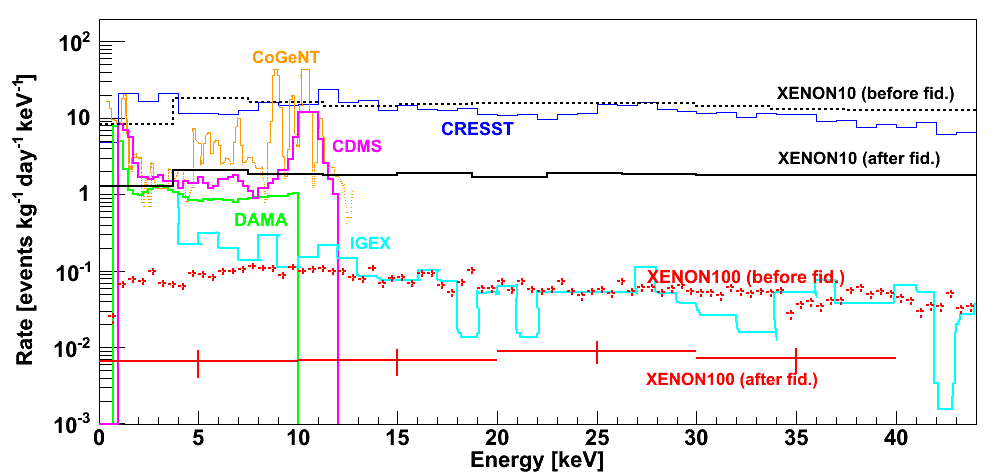
\includegraphics[width=1.0\linewidth]{plots/Xe1T/comparison_withLabels_wide.png}
\caption[Electronic recoil background of the XENON100 detector, compared to backgrounds measured in other dark matter search experiments]{Electronic recoil background of the XENON100 detector, compared to backgrounds measured in other dark matter search experiments. The plot is only indicative at low energies, since there is no calibration of the electronic recoil energy scale for liquid xenon detectors below 9~keV$_{\mathrm{ee}}$.}
\label{figXe100_BGcomparison}
\end{figure}

All photomultiplier tubes have been tested before the installation in the detector, in order to determine their functionality, avoid possible failure, and arrange them within the detector according to their measured characteristics. A system for the PMT gain calibration has been developed, including the hardware setup for the stimulation of the photoelectron emission with an external light source, and the software for the raw data processing and analysis of the single photoelectron response. The PMT calibration is performed regularly, typically once per week. A dynamic database and a web-based visualization tool allow for the correct processing and analysis of the measured data, and for the monitoring of the time evolution of the various quantities that characterize the detector stability.

The response of XENON100 has been studied with various calibration sources. A combined energy scale, providing improved linearity and resolution, has been studied for the lines with different energies, and was used for a spectroscopy analysis of the measured spectra.

Prompt (S1) and proportional light (S2) collection have been modeled with Monte Carlo simulations, and show a good agreement with the measurements. The collection efficiency, determined on the measured data as a function of the event vertex, provides spatial corrections for the measured S1 and S2 signals, which significantly improve the energy resolution of the detector. An $XY$ vertex reconstruction algorithm has been developed using a neural network for pattern recognition, which provides millimeter reconstruction precision. Its performance has been extensively validated on the measured and simulated data and has been compared with the expectations.

Sources of electromagnetic recoil background in XENON100 have been identified and modeled with GEANT4 based on the precise geometry of the experiment. The results from radioactive screening of the detector and shield materials and background measurements with delayed coincidence analyses have been taken into account. The predicted electronic recoil background rate and its energy spectrum are in a very good agreement with the measurements. The results of this study have been published in Ref.~\cite{EMBG}.

The innovative design with the careful selection of materials in terms of radioactive purity and an active liquid xenon veto surrounding the target volume results in the ultra-low background device for particle detection. The precise event vertex reconstruction allows to fiducialize the LXe target, reducing the electronic recoil background down to $<$10$^{-2}$~events$\cdot$kg$^{-1}\cdot$day$^{-1}\cdot$keV$^{-1}$, which is the lowest level achieved by existing dark matter search experiments, as shown in Fig.~\ref{figXe100_BGcomparison}.

\begin{figure}[!b]
\centering
\subfigure[]{
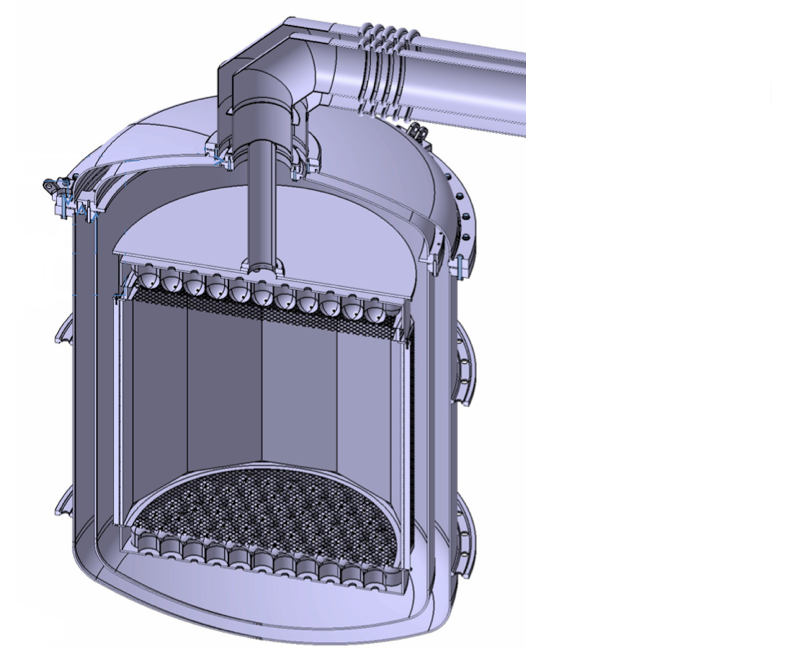
\includegraphics[height=0.35\linewidth]{plots/Xe1T/Xe1T_cryostat1.png}
\label{figXe1T_1}}
\subfigure[]{
\includegraphics[height=0.35\linewidth]{plots/Xe1T/Xe1t_tank.png}
\label{figXe1_2}}
\caption[Possible design of the XENON1T experiment]{Possible design of the XENON1T experiment. The titanium cryostat is immersed in a large water tank equipped with photosensors, which acts as a passive veto against external electromagnetic and neutron backgrounds, and as a muon veto.}
\label{figXe1T}
\end{figure}

The most critical background in direct dark matter searches, however, is due to neutrons, which interact in the same way as expected from a WIMP. Hence, the neutron production in ($\alpha$,n) and spontaneous fission reactions due to radioactive contamination in the detector materials has been calculated. The nuclear recoil background from radiogenic and cosmogenic (muon-induced) neutrons has been predicted with Monte Carlo simulations. This background source currently does not limit the detector sensitivity for WIMP detection.

First results from XENON100, obtained with only 11.2 live days of data acquired during a commissioning run~\cite{xe100-run07}, have shown a sensitivity competitive with that from the full exposure of CDMS-II~\cite{CDMS_limit},  demonstrating the potential of the experiment to discover WIMP dark matter. The result of the analysis of the first science run (100~live days)~\cite{xe100-run08} excludes a large fraction of previously unexplored WIMP parameter space, and cuts into the region where supersymmetric WIMP dark matter is accessible by the LHC~\cite{LHC}. The achieved limit on spin-independent WIMP-nucleon scattering cross-section challenges the interpretation of the DAMA~\cite{DAMA_LightWIMP} and CoGeNT~\cite{CoGeNT_LightWIMP} signals as being due to light mass WIMPs.

At the time of writing, the next phase of the XENON dark matter search program, XENON1T, is already being designed. It will use a target mass of $\sim$2.5 tons, and aims for a background goal of 10$^{-4}$ events$\cdot$kg$^{-1}\cdot$day${-1}\cdot$keV$^{-1}$, about a factor of 100 lower than that in XENON100. It will  provide the sensitivity to detect WIMPs in most of the theoretically favored parameter space, probing spin-independent WIMP-nucleon scattering cross sections down to 2$\times$10$^{-47}$~cm$^{2}$. A preliminary drawing of the XENON1T detector is shown in Fig.~\ref{figXe1T}. The titanium cryostat will be immersed in a water tank equipped with photosensors, which will act as a passive veto against external $\gamma$ and neutron backgrounds, and as an active muon veto. This design will allow to significantly reduce the electromagnetic background from external sources, and the dominant background source will be $^{85}$Kr in the liquid xenon target. Figure~\ref{figXe1Tsensitivity} compares the predicted energy spectra from this background source with the spectra of a 100~GeV/c$^{2}$ WIMP, scaled to the expected sensitivity of the XENON100 experiment~\cite{xe100-projection} of 2$\times$10$^{-45}$~cm$^{2}$, and the expected sensitivity of XENON1T (2$\times$10$^{-47}$~cm$^{2}$), assuming 99.5\% electronic recoil discrimination. The krypton concentration of $\sim$100~ppt achieved in XENON100 is well above the WIMP spectrum expected for $\sigma$ = 2$\times$10$^{-47}$~cm$^{2}$. Therefore, it has to be reduced to $\sim$1~ppt in order not to be a limitation for the experiment. This krypton concentration will then result in a background level similar to that from pp solar neutrinos, also shown in the plot.

\begin{figure}[!h]
\centering
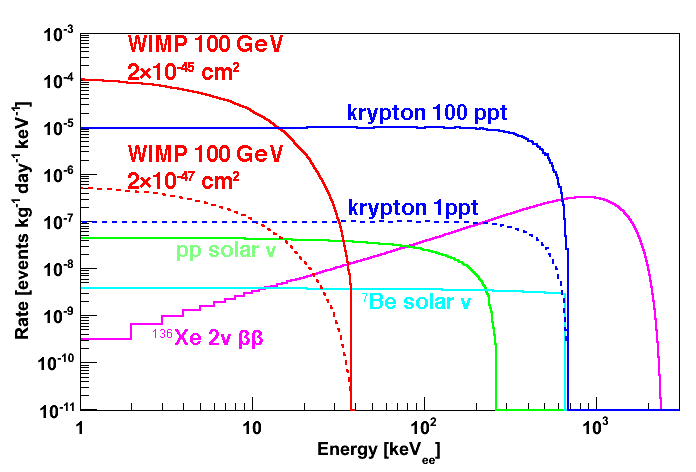
\includegraphics[width=0.6\linewidth]{plots/Xe1T/Xe100andXe1Tsensitivity_with100ppt_withLabels.png}
\caption[Projected sensitivity of the XENON1T experiment]{The planned cross section sensitivity of the XENON100 experiment (2$\times$10$^{-45}$~cm$^{2}$ for a 100~GeV/c$^{2}$ WIMP) and the expected sensitivity for XENON1T (2$\times$10$^{-47}$~cm$^{2}$). The reduction of krypton concentration down to $\sim$1~ppt is required to achieve this goal. The corresponding background level, assuming 99.5\% electronic recoil discrimination, is similar to that expected from pp solar neutrinos. The predicted energy spectra of pp and $^{7}$Be solar neutrinos are plotted using the shape from Ref.~\cite{SolarNeutrinoSpectra} and the fluxes calculated in Ref.~\cite{SolarNeutrinoFlux}. The 2$\nu$ $\beta\beta$ decay of $^{136}$Xe is also shown, using the current half-life time limit of 1.1$\times$10$^{22}$~years from Ref.~\cite{DoubleBetaLimitDAMA}.}
\label{figXe1Tsensitivity}
\end{figure}

